%\documentclass[12pt,a4paper]{article}
\documentclass[rgb,pdftex, oneside, fontsize=12pt,chapterprefix,cleardoublepage=empty,listof=totoc,bibliography=totoc,numbers=noenddot,headsepline,%footsepline,footinclude=false,headinclude=false
]{memoir}
\usepackage{import}
\linespread{1.3}\selectfont

%%%%%%%%%%%%%%%%%%%%%%%%%%%%%%%%%%%%%%%%%%%%%%%%%%%%%%%%%%%%%%%%%%%%%%%%%%
%%% JKU Wirtschaftsinformatik Thesis template                          %%%
%%% Daniel Lehner, Institut fuer Wirtschaftsinformatik, Jun 2022       %%
%%% Coversheet by: Andreas Neubauer, May 2016                          %%%    
%%%%%%%%%%%%%%%%%%%%%%%%%%%%%%%%%%%%%%%%%%%%%%%%%%%%%%%%%%%%%%%%%%%%%%%%%%
%CONFIG-PROPERTY 1: Degree: select your degree                         %%%
%CONFIG-PROPERTY 2: Cover Sheet Info: supervisor, etc.                 %%%
%%%%%%%%%%%%%%%%%%%%%%%%%%%%%%%%%%%%%%%%%%%%%%%%%%%%%%%%%%%%%%%%%%%%%%%%%%

%\chapterstyle{veelo}


% Set PDF document properties
\hypersetup{
    pdfpagelayout   = TwoPageRight
}

%\setsecnumdepth{subsection} % Enumerate subsections.

%\nonzeroparskip             % Create space between paragraphs (optional).
\setlength{\parindent}{0pt} % Remove paragraph identation (optional).



%%%%%%%%%%%%%%%%%%%%%%%%%%%%%%%%%%%%%%%%%
%%% Some useful macros for section,   %%%
%%% figure, and table referencing...  %%%

%%%%%%%%%%%%%%%%%%%%%%%%%%%%%%%%%%%%%%%%%
\newcommand{\citechap}[1]{Chapter~\ref{chap:#1}}
\newcommand{\citesec}[1]{Section~\ref{sec:#1}}
\newcommand{\citefig}[1]{Fig.~\ref{fig:#1}}
\newcommand{\citealgo}[1]{\textsc{Listing}~\ref{algo:#1}}
\newcommand{\citelisting}[1]{\textsc{Listing}~\ref{lst:#1}}
\newcommand{\citetable}[1]{{Table}~\ref{tab:#1}}
 \newcommand{\etal}{\latinphrase{et~al.}\xspace}
\newcommand{\ie}{\latinphrase{i.e.}\xspace}


%%%%%%%%%%%%%%%%%%%%%%%%%%%%%%%%%%%%%%%%%
%%% some colors                       %%%
%%%%%%%%%%%%%%%%%%%%%%%%%%%%%%%%%%%%%%%%%

\definecolor{pink}{rgb}{0.9,0,0.9}
\definecolor{gray}{rgb}{0.95,0.95,0.85}
\definecolor{mauve}{rgb}{0.1,0.7,0.2}
\definecolor{bg}{rgb}{0.95,0.95,0.9} 
\definecolor{dkgreen}{rgb}{0,0.6,0}

\newcommand{\note}[1]{\textbf{\textcolor{purple}{#1}}}
\newcommand{\commnt}[1]{\textbf{\textcolor{dkgreen}{#1}}}  


%%%%%%%%%%%%%%%%%%%%%%%%%%%%%%%%%%%%%%%%%
%%%  Header / Footer configuration   %%%% 
%%%%%%%%%%%%%%%%%%%%%%%%%%%%%%%%%%%%%%%%%
 \clearscrheadfoot
%\pagestyle{scrheadings}

\rofoot[\pagemark]{\pagemark}
\lefoot[\pagemark]{\pagemark}

\selectlanguage{american}

%%%%%%%%%%%%%%%%%%%%%%%%%%%%%%%%%%%%%%%%%
%%%%%%%%%%%% CONFIG-PROPERTY 1: %%%%%%%%%
%%%% Degree                          %%%% 
%%%% Select your degree type          %%%
%%%%%%%%%%%%%%%%%%%%%%%%%%%%%%%%%%%%%%%%%

%% Master/Bacc Studium - e.g.:
%\def\degree{Bachelor of Science}
%\def\degree{Master of Science}
%\def\degree{Diplom-Ingenieur}

% e.g. Doktorratsstudium - e.g.:
%\def\degree{Doktor der technischen Wissenschaften}
\def\degree{Doktor der Sozialwissenschaften}


%%%%%%%%%%%%%%%%%%%%%%%%%%%%%%%%%%%%%%%%%
%%%%%%%%%%%% CONFIG-PROPERTY 2: %%%%%%%%%
%%%% Cover sheet info                %%%% 
%%%% Enter your details here          %%%
%%%%%%%%%%%%%%%%%%%%%%%%%%%%%%%%%%%%%%%%%

\newcommand{\institute}{Institut für\\ Wirtschaftsinformatik\\Software Engineering}
\newcommand{\thtitle}{Thesis Title}
\newcommand{\name}{Name}
\newcommand{\supervisor}{First Supervisor}
\newcommand{\secondexaminer}{Second Examiner}
\newcommand{\assist}{Co-Supervisor}
\newcommand{\submitted}{10 2019}
\newcommand{\study}{Sozial- und Wirtschaftswissenschaften}

\setcounter{subsection}{1}
\setcounter{section}{1}

\usepackage[a4paper,width=150mm,top=35mm,bottom=50mm,outer=20mm, inner=35mm,]{geometry}
\begin{document}
\frontmatter % Switches to roman numbering.

%%%%%%%%%%%%%%%%%%%%%%%%%%%%%%%%%%%%%%%%%
%%%% Coverpage, don't change...      %%%% 
%%%%%%%%%%%%%%%%%%%%%%%%%%%%%%%%%%%%%%%%%

\pagestyle{empty}
% \newgeometry{top=20mm,bottom=40mm,textwidth=16.7cm,left=20mm,right=-20mm}
\afterpage{\aftergroup\restoregeometry}
%%Andreas Neubauer, May 2016
\textwidth 16.7cm
\textheight 25cm
\topmargin -2.7cm
\oddsidemargin 0.25cm
\parindent 0pt
\pagestyle{empty}
%
% -------- only change entries beginning here ----------------------------
%
% choose language of coverpage: german or english
%\newif\ifeng
%\engtrue
%\engfalse
%


%
% enter the study (Studienrichtung, as stated in your curriculum)
%
% e.g. Diplomstudium:
%\def\study{Lehramt Mathematik}
%
% e.g. Masterstudium:
%\def\study{Industriemathematik}
%
% e.g. Doktorratsstudium
%\def\study{Technische Wissenschaften}
%\def\study{Naturwissenschaften}
%
%

% enter the name of the supervisor and first thesis examiner
% only for type 0 (Dissertation) you need a second thesis examiner
% 
% for the german version you also have to enter the sex (male or female)
% of the supervisor/examiners
%
\newif\ifsupvismale
\supvismaletrue
%\supvismalefalse
%
\def\secondexaminer{Name of 2. examiner}
\newif\ifsecexmale
\secexmaletrue
%\secexmalefalse
%
% enter month year
% (the month when you brought it to the Prüfungs- und Anerkennungsservice)
%
%
% do not change anything below this line
% -------------------------------------------------------------------------------
%
\def\ifundefined#1{\expandafter\ifx\csname#1\endcsname\relax}
\DeclareFontShape{OT1}{cmss}{m}{n}
  {<5><6><7><8><9><10><10.95><12><14.4><17.28><20.74><24.88><29.86><35.83>%
   <42.99><51.59><67><77.38>cmss10}{}
\DeclareFontShape{OT1}{cmss}{bx}{n}
  {<5><6><7><8><9><10><10.95><12><14.4><17.28><20.74><24.88><29.86><35.83>%
   <42.99><51.59><67><77.38>cmssbx10}{}
\makeatletter
\def\Huge{\@setfontsize\Huge{29.86pt}{36}}
\makeatother
%
\unitlength 1cm
\sffamily
\begin{picture}(16.7,0)
\ifeng
 \put(11.5,-2.5){
\includegraphics[width=5.2cm]{figures/cover/jku_en}}
\else
 \put(11.5,-2.5){
\includegraphics[width=5.2cm]{figures/cover/jku_de}}
\fi
\put(12.9,-4.2){\begin{minipage}[t]{3.9cm}\footnotesize%
\ifeng
 Submitted by\\
\else
 Eingereicht von\\
\fi
{\bfseries\name}%
\vskip 4mm%
\ifeng
 Submitted at\\
\else
 Angefertigt am\\
\fi
{\bfseries\institute}%
\vskip 4mm%
\ifcase\type%
 \ifeng
  Supervisor and\\ First Examiner\\
 \else
  \ifsupvismale%
   Betreuer und\\ Erstbeurteiler\\
  \else
   Betreuerin und\\ Erstbeurteilerin\\
  \fi
 \fi
 {\bfseries\supervisor}%
 \vskip 4mm%
 \ifeng
  Second Examiner\\
 \else
  \ifsecexmale%
   Zweitbeurteiler\\
  \else
   Zweitbeurteilerin\\
  \fi
 \fi
 {\bfseries\secondexaminer}%
\else
 \ifeng
  Supervisor\\
 \else
  \ifsupvismale%
   Betreuer\\
  \else
   Betreuerin\\
  \fi
 \fi
 {\bfseries\supervisor}%
\fi
\vskip 4mm%
\ifundefined{assist}\else
 \ifeng
  Co-Supervisor\\
 \else
  Mitbetreuung\\
 \fi
 {\bfseries\assist}%
\vskip 4mm%
\fi
\submitted
\end{minipage}}
\put(12.9,-25){\begin{minipage}[t]{3.9cm}\footnotesize%
{\bfseries JOHANNES KEPLER\\
\ifeng
 UNIVERSITY
\else
 UNIVERSIT\"AT
\fi
LINZ}\\
Altenbergerstra{\ss}e 69\\
4040 Linz, \"Osterreich\\
www.jku.at\\
DVR 0093696
\end{minipage}}
\put(0,-12.2){\begin{minipage}[b]{12cm}\Huge\bfseries\thtitle\end{minipage}}
\put(0,-17.2){
\includegraphics[width=4.4cm]{figures/cover/arr}}
\put(0,-18.3){\begin{minipage}[t]{12cm}%
\ifeng
 {\large\ifcase\type Doctoral \or Diploma \or Master \or Bachelor \fi Thesis}%
 \vskip 2mm%
 to obtain the academic degree of%
 \vskip 3mm%
 {\large\degree}
 \vskip 3mm%
 in the \ifcase\type Doctoral \or Diploma \or Master's \or Bachelor's \fi Program
\else
 {\large\ifcase\type Dissertation\or Diplomarbeit\or Masterarbeit \or Bachelorarbeit \fi}%
 \vskip 2mm%
 zur Erlangung des akademischen Grades%
 \vskip 3mm%
 {\large\degree}
 \vskip 3mm%
 im \ifcase\type Doktoratsstudium \or Diplomstudium\or Masterstudium \or Bachelorstudium \fi
\fi
\vskip 3mm%
{\large\study}
\end{minipage}}
\end{picture}

\setcounter{page}{1}
\frontmatter
\pagestyle{scrheadings}

\renewcommand{\bibname}{References}
\renewcommand{\contentsname}{Table of Contents} 


%%%%%%%%%%%%%%%%%%%%%%%%%%%%%%%%%%%%%%%%%
%%%% Content goes here:              %%%% 
%%%%%%%%%%%%%%%%%%%%%%%%%%%%%%%%%%%%%%%%%




\chapter*{Abstract}
Insert abstract (english) here...

\tableofcontents*


\chapter{Introduction}
\label{chap:introduction}
Describe the research problem statement, with proper motivations

\cite{Turing1936}
\section{Latex Examples}

\subsection{Headings}
Sections, sub-sections and sub-sub-sections allow different levels of headings. 
This can be done via the \verb|\section|, \verb|\subsection|, and \verb|\subsubsection| command respectively.
Try to avoid more than 3 levels of headings in your paper!


\subsection{Include files}
If sections are split in several .tex files they can be included via the  \verb|\input | command respectively.
For example:  \verb|\section{Introduction}
\label{sec:introduction}


\lipsum[1-3] \cite{Turing1936}
\begin{figure}[h!]
\centering
  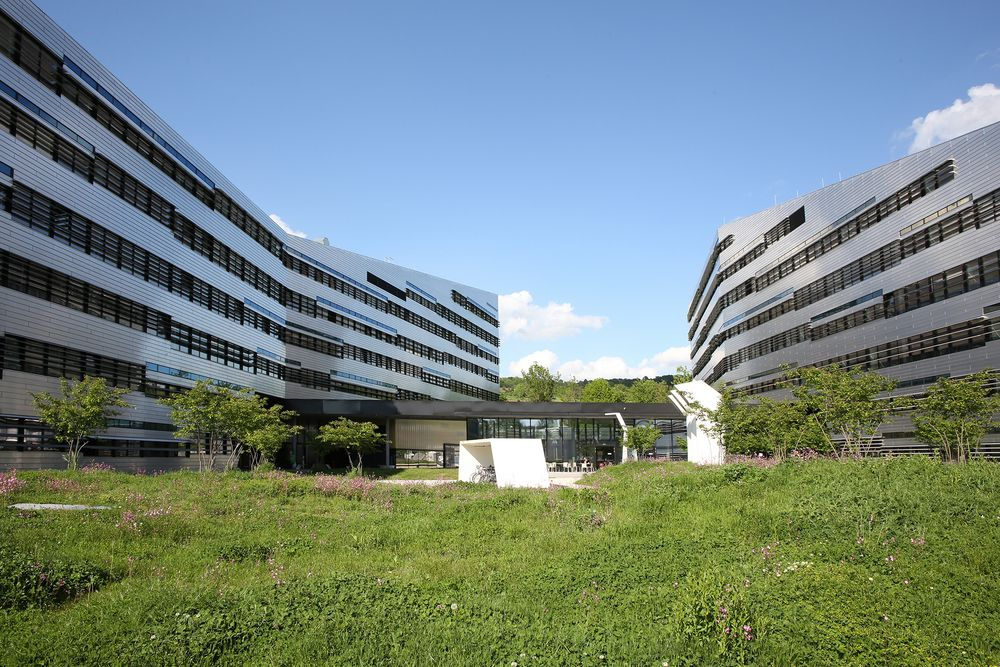
\includegraphics[width=0.8\linewidth]{figures/science_park.jpg}
  \caption{A boat.}
  \label{fig:boat1}
\end{figure}
\lipsum[4-6] | adds the introduction.tex file.  \verb|\input{chapters/chapter1}| would add the chapter1.tex file from the chapters folder. 


\subsubsection{A sub-subsection}

\subsection{Items and Enumerations}
 The environment \verb|\itemize| allows to create a lists whereas the environment \verb|\enumerate| creates a numbered list. Both environments are created via the \verb|\begin{itemize}| and \verb|\end{itemize}| or  \verb|\begin{enumerate}| and \verb|\end{enumerate}| commands.\\
 
 An unordered list:
\begin{itemize}
  \item An Item
  \item Another Item
  \item Yet another Item
\end{itemize}

 An ordered list:
\begin{enumerate}
  \item One
  \item Two
  \item Three
\end{enumerate}

\subsection{Citations}

Latex uses the BibTEX reference management software which allows to cite references using the \verb|\cite| command.
For example~\cite{Turing1936}.


\subsection{Referencing Sections, Figures, and Tables}

References to different items can be created via the  \verb|\ref|.
The items need to be labeled with the \verb|\label| command.

For example, a section labeled with  \verb|\label{sec:introduction}| can be referenced with\newline \verb|\ref{sec:introduction}|. This generates the respective number: ``In section~\ref{sec:introduction} \ldots''\\

\bigskip
We provide a couple of custom commands to make it easier to reference tables, figures and sections that automatically adds the section, table or figure prefix: 

\begin{itemize}
    \item \verb|\citesec|:    ``In~\citesec{introduction} \ldots''
    \item \verb|\citefig|:    ``In~\citefig{sample-fig} \ldots''
    \item \verb|\citetable| : ``In~\citetable{example} \ldots''

\end{itemize}



\subsection{Figures}

An image is added to a document via the \verb|\includegraphics| for jpg, png, or pdf images  or with \verb|\includesvg| for vector images ans shown in \citefig{sample-fig}

\begin{figure}[h!]
\centering
  %
\includegraphics[width=0.8\linewidth]{figures/sample-figure.png}
   \includesvg[width=0.5\linewidth]{figures/sample-figure.svg}
  \caption{A sample svg image}
  \label{fig:sample-fig}
\end{figure}


\subsection{Tables}



A table in \LaTeX\ is created by using a \verb|tabular| environment or any of its extensions, e.g., \verb|tabularx|.
\citetable{example} shows an example of a simple table.

\begin{table}[th!]
\centering
\begin{tabular}{p{4cm}r}
\toprule
Category                & Wind	Speed (Mph)             \\ \midrule
1                       & 25                            \\
2                       & 25                            \\
3                       & 25                            \\ \midrule
4                       & 25                            \\
5                       & \textgreater{}=155           \\ \bottomrule
\end{tabular}
 \caption{The caption of the table}\label{tab:example}
\end{table}






%%%%%%%%%%%%%%%%%%%%%%%%%%%%%%%%%%%%%%%%%
%%% List of tables, figures,         %%%%
%%% references...                    %%%% 
%%%%%%%%%%%%%%%%%%%%%%%%%%%%%%%%%%%%%%%%%




% Add a glossary.
\printglossaries

%%%%%%%%%%%%%%%%%%%%%%%%%%%%%%%%%%%%%%%%%
%%%% Select bibliography style       %%%%
%%%%%%%%%%%%%%%%%%%%%%%%%%%%%%%%%%%%%%%%%
%\bibliographystyle{abbrv}
%\bibliographystyle{apalike}
\bibliographystyle{alpha}
\bibliography{references}




\end{document}